%!TEX program = xelatex

\documentclass[11pt,titlepage]{report}
%!TEX root = main.tex

\usepackage[T1]{fontenc}
\usepackage{lmodern}
\usepackage[svgnames]{xcolor}
\usepackage{fontspec} % XeLaTeX required!
\usepackage{graphicx}
\usepackage{circuitikz}
\usepackage{tikz}
\usepackage{pifont}
\usepackage[some]{background}
\usepackage{xltxtra} 
\usepackage{setspace}
\usepackage[absolute]{textpos}
\usepackage[latin1]{inputenc}
\usepackage[english]{babel}
\usepackage{graphicx}
\usepackage{wrapfig}
\usepackage{fullpage}
\usepackage[margin=1in]{geometry}
\usepackage{float}
\usepackage{url}
\usepackage{multicol}
\usepackage{hyperref}
\usepackage{titlepic}
\usepackage{standalone}
\usepackage{siunitx}
\usepackage{booktabs}
\usepackage{amsmath}
\usepackage{unicode-math}
\usepackage{verbatim}
\usepackage{enumitem}
\usepackage{listings}
\usepackage{multirow}
\usepackage{pgfplots}
\pgfplotsset{compat=1.8}
\usepackage{caption} 
\usepackage[parfill]{parskip}
\usepackage{import}
\usepackage[backend=bibtexu,texencoding=utf8,bibencoding=utf8,style=ieee,sortlocale=en_GB,language=auto]{biblatex}
\usepackage[strict,autostyle]{csquotes}
\usepackage[final]{pdfpages}
\usepackage{subcaption}
\usepackage{ifplatform}
%\captionsetup[table]{skip=10pt}


% Fix for includepdf bug in Mac OS X
\newcommand{\insertpdfpath}[1]{
	\ifwindows
	\newcommand{\insertpdf}[2]{\includepdf[pages=##1]{##2}}
	\else
	\newcommand{\insertpdf}[2]{\includepdf[pages=##1]{#1/##2}}
	\fi
}

%set fonts
\setmainfont[Ligatures=TeX]{Myriad Pro}
\setmathfont{Asana Math}
\setmonofont{Lucida Console}

\usepackage{titlesec, color}
\renewcommand{\familydefault}{\sfdefault} %set font family
\renewcommand{\arraystretch}{1.2} %set table vertical spacing
\setlength\parindent{0pt} %no paragraph indent
\hypersetup{ %setup hyperlinks
    colorlinks,
    citecolor=black,
    filecolor=black,
    linkcolor=black,
    urlcolor=black
}

%redesign chapter headings
\definecolor{gray75}{gray}{0.75}
\newcommand{\chapternumber}{\thechapter}
\newcommand{\hsp}{\hspace{20pt}}
\titleformat{\chapter}[hang]{\Huge\bfseries}{\chapternumber\hsp\textcolor{gray75}{|}\hsp}{0pt}{\Huge\bfseries}

%Redefine appendix headers
\renewcommand{\appendixname}{Appendix}
\renewcommand{\appendixtocname}{Appendices}
\renewcommand{\appendixpagename}{Appendices}

%For code listings
\definecolor{black}{rgb}{0,0,0}
\definecolor{browntags}{rgb}{0.65,0.1,0.1}
\definecolor{bluestrings}{rgb}{0,0,1}
\definecolor{graycomments}{rgb}{0.4,0.4,0.4}
\definecolor{redkeywords}{rgb}{1,0,0}
\definecolor{bluekeywords}{rgb}{0.13,0.13,0.8}
\definecolor{greencomments}{rgb}{0,0.5,0}
\definecolor{redstrings}{rgb}{0.9,0,0}
\definecolor{purpleidentifiers}{rgb}{0.01,0,0.01}


\lstdefinestyle{csharp}{
language=[Sharp]C,
showspaces=false,
showtabs=false,
breaklines=true,
showstringspaces=false,
breakatwhitespace=true,
escapeinside={(*@}{@*)},
columns=fullflexible,
commentstyle=\color{greencomments},
keywordstyle=\color{bluekeywords}\bfseries,
stringstyle=\color{redstrings},
identifierstyle=\color{purpleidentifiers},
basicstyle=\ttfamily\small}

\lstdefinestyle{c}{
language=C,
showspaces=false,
showtabs=false,
breaklines=true,
showstringspaces=false,
breakatwhitespace=true,
escapeinside={(*@}{@*)},
columns=fullflexible,
commentstyle=\color{greencomments},
keywordstyle=\color{bluekeywords}\bfseries,
stringstyle=\color{redstrings},
identifierstyle=\color{purpleidentifiers},
}

\lstdefinestyle{matlab}{
language=Matlab,
showspaces=false,
showtabs=false,
breaklines=true,
showstringspaces=false,
breakatwhitespace=true,
escapeinside={(*@}{@*)},
columns=fullflexible,
commentstyle=\color{greencomments},
keywordstyle=\color{bluekeywords}\bfseries,
stringstyle=\color{redstrings},
identifierstyle=\color{purpleidentifiers}
}

\lstdefinestyle{vhdl}{
language=VHDL,
showspaces=false,
showtabs=false,
breaklines=true,
showstringspaces=false,
breakatwhitespace=true,
escapeinside={(*@}{@*)},
columns=fullflexible,
commentstyle=\color{greencomments},
keywordstyle=\color{bluekeywords}\bfseries,
stringstyle=\color{redstrings},
identifierstyle=\color{purpleidentifiers}
}

\lstdefinestyle{xaml}{
language=XML,
showspaces=false,
showtabs=false,
breaklines=true,
showstringspaces=false,
breakatwhitespace=true,
escapeinside={(*@}{@*)},
columns=fullflexible,
commentstyle=\color{greencomments},
keywordstyle=\color{redkeywords},
stringstyle=\color{bluestrings},
tagstyle=\color{browntags},
morestring=[b]",
  morecomment=[s]{<?}{?>},
  morekeywords={xmlns,version,typex:AsyncRecords,x:Arguments,x:Boolean,x:Byte,x:Char,x:Class,x:ClassAttributes,x:ClassModifier,x:Code,x:ConnectionId,x:Decimal,x:Double,x:FactoryMethod,x:FieldModifier,x:Int16,x:Int32,x:Int64,x:Key,x:Members,x:Name,x:Object,x:Property,x:Shared,x:Single,x:String,x:Subclass,x:SynchronousMode,x:TimeSpan,x:TypeArguments,x:Uid,x:Uri,x:XData,Grid.Column,Grid.ColumnSpan,Click,ClipToBounds,Content,DropDownOpened,FontSize,Foreground,Header,Height,HorizontalAlignment,HorizontalContentAlignment,IsCancel,IsDefault,IsEnabled,IsSelected,Margin,MinHeight,MinWidth,Padding,SnapsToDevicePixels,Target,TextWrapping,Title,VerticalAlignment,VerticalContentAlignment,Width,WindowStartupLocation,Binding,Mode,OneWay,xmlns:x}
}

\lstdefinestyle{matlab}{
language=Matlab,
showspaces=false,
showtabs=false,
breaklines=true,
showstringspaces=false,
breakatwhitespace=true,
escapeinside={(*@}{@*)},
columns=fullflexible,
commentstyle=\color{greencomments},
keywordstyle=\color{bluekeywords}\bfseries,
stringstyle=\color{purpleidentifiers},
identifierstyle=\color{purpleidentifiers}
}

%defaults
\lstset{
basicstyle=\ttfamily\small,
extendedchars=false,
numbers=left,
numberstyle=\ttfamily\tiny,
stepnumber=1,
tabsize=4,
numbersep=5pt
}
\addbibresource{../../library/bibliography.bib}

\begin{document}

\chapter{Assignment 3}
\section{Design}
The amount of power transferred to the load is desired to be as high as possible. One can see that by minimizing the impedance seen by a voltage source, the drawn power is maximized. It is therefore desired to compensate the impedance of the coils by making use of compensating capacitors. By equating the impedances of the coils and their capacitors, the capacitance of these capacitors can be calculated. This relationship is given by

\begin{equation}
\label{eq:ass3-compensation}
C = \frac{1}{(2 \pi f)^2 L}.
\end{equation}

Using Equation~\ref{eq:ass3-compensation} we obtain values of \SI{26.8}{nF} for the primary side and \SI{100.1}{nF} for the secondary side. Using a series combination of three times a parellel combination of two \SI{22}{nF} and one \SI{33}{nF} capacitor, all with a small deviation for the primary side and a parallel combination of a \SI{33}{nF} and a \SI{67}{nF} capacitor for the secondary side, we obtained real-world values of \SI{26.4}{nF} for de primary side and \SI{100.0}{nF} for the secondary side.

Expanding the model used in assignment 2 with the compensating capacitors we derive

\begin{equation} \label{eq:ass3-model-compensated}
	\mathbf{\vec{I}} \mathbf{Z}=
	\begin{bmatrix}
		I_{source} \\
		I_{load}
	\end{bmatrix}
	\begin{bmatrix}
		R_1 + j \omega L_1 + (j \omega C_1)^{-1}  & j \omega M\\
		j \omega M & R_2 + j \omega L_2 + (j \omega C_2)^{-1}  + R_L
	\end{bmatrix}
	= \mathbf{\vec{V}} =
	\begin{bmatrix}
		V_{source} \\
		0
	\end{bmatrix} .
\end{equation}

The values of the compensating capacitors are denoted by $C_1$ and $C_2$. The results of the simulation are displayed in Table~\ref{tab:ass3-power-sim}.

\begin{table}[H]
	\centering
	\caption{Power transfer simulations - compensated}
	\label{tab:ass3-power-sim}
	\begin{tabular}{c c c c c c c}
		\hline\hline
		Distance & Source voltage & Source current & Source power & Load voltage & Load power & Efficiency \\
		\hline
		\SI{0}{cm} & \SI{20}{V} & \SI{0.5353}{A} & \SI{10.70}{W} & \SI{10.32}{V} & \SI{10.38}{W} & \SI{97}{\percent} \\
		\SI{2}{cm} & \SI{20}{V} & \SI{1.9639}{A} & \SI{39.27}{W} & \SI{19.59}{V} & \SI{37.39}{W} & \SI{95}{\percent} \\
		\SI{4}{cm} & \SI{20}{V} & \SI{5.6343}{A} & \SI{112.68}{W} & \SI{32.27}{V} & \SI{101.46}{W} & \SI{90}{\percent} \\
		\SI{6}{cm} & \SI{20}{V} & \SI{9.4482}{A} & \SI{188.96}{W} & \SI{38.86}{V} & \SI{147.18}{W} & \SI{78}{\percent} \\
		\hline
		\end{tabular}
\end{table}

Rewriting Equation~\ref{eq:ass3-model-compensated} results in the transfer function given by

\begin{equation} \label{eq:ass3-transfer-function}
	|H(s)| = \frac{s M Z_L}{(s M)^2 - (s L_2 + R_2 + (s C_2)^{-1} + Z_L) ( s L_1 + R1 + (s C_1)^{-1}))} .
\end{equation}

\begin{figure}[H]
	\begin{center}
		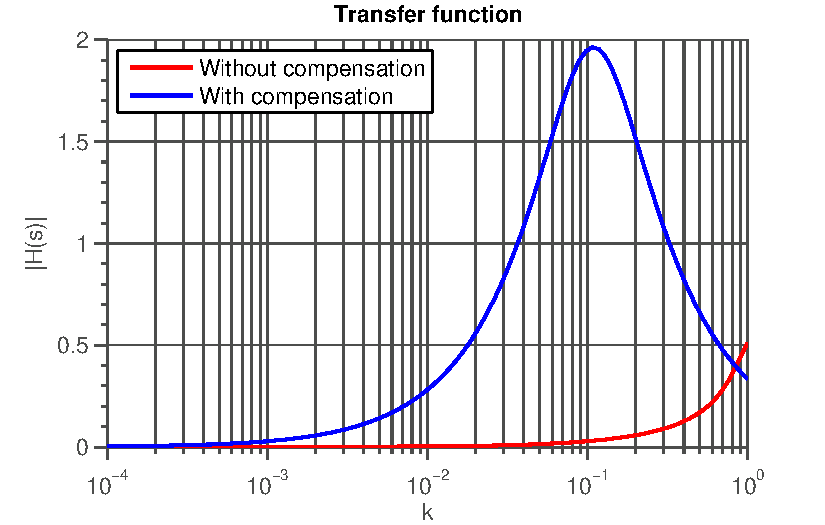
\includegraphics[width=0.8\linewidth]{resource/transfer_function-rc.pdf}
	\end{center}
	\caption{Transfer function with and without compensation}
	\label{fig:ass3-transfer-function}
\end{figure}

Graphically evaluating Equation~\ref{eq:ass3-transfer-function} results in Figure~\ref{fig:ass3-transfer-function}. It is clear that one can maximize the power transfer after adding the compensating capacitors. This optimum is an equilibrium between the losses of the increasing leakage inductances and increased power drawn from the voltage source. The power drawn from the voltage source is proportional to the current drawn. The current drawn is proportional to the impedance seen by the voltage source, which decreases if the mutual inductance decreases. Therefore, the power drawn increases if the mutual inductance decreases.

\section{Results}
To test our design, we studied its waveforms using the oscilloscope. Screenshots of this are included in Appendix~\ref{}. 
%TODO add screenshots to appendix and insert reference
From this waveforms may be concluded that the inverter will generate a correct DC-signal when rectified.
%TODO insert actual rectified output screenshot
We also performed the same power transfer measurements as with the uncompensated converter, whose results are displayed in Table~\ref{tab:ass3-power}.

\begin{table}[H]
	\centering
	\caption{Power transfer measurements - compensated}
	\label{tab:ass3-power}
	\begin{tabular}{c c c c c c c}
		\hline\hline
		Distance & Source voltage & Source current & Source power & Load voltage & Load power & Efficiency \\
		\hline
		\SI{2}{cm} & \SI{19.998}{V} & \SI{1.2472}{A} & \SI{24.942}{W} & \SI{14.8}{V} & \SI{21.3}{W} & \SI{85.6}{\percent} \\
		\hline
		\end{tabular}
\end{table}

If we compare these results with Table~\ref{tab:ass2-power} from the uncompensated converter, we see that the delivered power is more than fifty times higher, while the efficiency more than tripled. However, the measured values deviate a lot from the simulated values. This is due to the sensibility of the setup to external factors, such as mechanical placement. With the compensated converter, charging the supercapacitor bank took us little under three minutes.

\section{Questions}
\begin{enumerate}
\item
Performing Fourier analysis to a square wave reveals that the fundamental sinus, which is a sinus with the same frequency of the square, is most influential. The system we are analysing is linear. Therefore, we can conclude that the reponse to the square wave can be approximated by the reponse to its fundamental sinus.

\item
%The imaginary part of both of the converter's sides should equal zero. This way power transfer is maximized, because leakage inductances are compensated for, thus the power factor is increased. This can be accomplished by compensating both coils with a capacitance.
In a voltage oriented system, the power transfer can be maximized by maximizing the current. By compensating the impedance of the coils, we can minimize the impedance seen by the voltage source and consequently maximize the power transfer.
% TODO: choose one of the two explanations

\item
When the secondary coil is not present, the equivalent circuit reduces to a single loop with a tiny resistance, capacitance and inductance. Since the capacitance and inductance are designed to be in resonance, the impedance of the loop is very low. This allows for a very high current to flow, which could overload the converter and its power source.

\item
To overcome this problem an overcurrent protection circuit is built in. This circuit measures the voltage over a shunt resistance and compares this to a reference voltage. When the shunt voltage (and thus the source current) exceeds the reference voltage, the circuit will trigger via positive feedback (being a Schmitt-trigger), so the output of the circuit becomes a logical `1'. This output signal is connected to the UC3525's \textit{shutdown}-input, so it will stop generating the PWM-signal. This way the converter is turned off, until the reset button is pressed.
%TODO check this + estimate maximum current
\end{enumerate}
\end{document}